\documentclass[11pt,a4paper,titlepage]{article}
\oddsidemargin 0.2in 
\evensidemargin 0.2in
\textwidth 6.0in
\usepackage[utf8]{inputenc}
\usepackage[T1]{fontenc}
\usepackage{lmodern}
\usepackage[english]{babel}
\usepackage[tbtags]{amsmath}
\usepackage{wasysym}
\usepackage{amssymb}
\usepackage{graphicx}
\usepackage{epic}
\usepackage{eepic}
\usepackage{multicol}
\usepackage{fancyhdr}
\usepackage{float}
\usepackage{fancybox}
\usepackage{subfig}
\usepackage{endnotes}
\usepackage{natbib}		% REFERENCER FORMATERET SOM NATURVIDENSKAB
\usepackage{latexsym} 
% \usepackage{feynmf}		%Package for feynman diagrams.
\usepackage{axodraw4j} % Packages for JaxoDraw
\usepackage{pstricks}
\usepackage{color}

% % % % % % % % % % % % % % % % Bra-Ket % % % % % % % % % % % % % % % %

\newcommand{\ket}[1]{
  |#1 \rangle
}

\newcommand{\bra}[1]{
  \langle #1|
}

\newcommand{\braket}[2]{
  \langle #1|#2 \rangle
}

% % % % % % % % % % % % % % % % FIGURER % % % % % % % % % % % % % % % %
\newcommand{\includefigure}[4]{
\begin{figure}[htbp] \centering
		\includegraphics[scale=#2]{#3}
		\caption{\footnotesize #4}
		\label{#1}
\end{figure}
}
% % % % % % % % % % % % % % OPSKRIFT PAA EN FIGUR % % % % % % % % % % % %

%\includefigure{NAVN_PAA_FIGUREN}{FIGURENS STORRELSE (0-1)}{FILNAVN}{FIGURTEKST}

% % % % % % % % % % % % % % % REFERENCER % % % % % % % % % % % % % % %
\renewcommand\notesname{Referencer}
\numberwithin{equation}{section}

%----Different font in captions----
\newcommand{\captionfonts}{\small}

\makeatletter  % Allow the use of @ in command names
\long\def\@makecaption#1#2{%
  \vskip\abovecaptionskip
  \sbox\@tempboxa{{\captionfonts #1: #2}}%
  \ifdim \wd\@tempboxa >\hsize
    {\captionfonts #1: #2\par}
  \else
    \hbox to\hsize{\hfil\box\@tempboxa\hfil}%
  \fi
  \vskip\belowcaptionskip}
\makeatother   % Cancel the effect of \makeatletter
%------------Define Keys-------------

\makeindex

\parskip        =    1ex
\parindent      =    0em
\baselineskip   =    2ex

% % % % % % % % % %% % % % % FANCY SHIZZLE? % % % % % % % % % % % % % % %
\pagestyle{fancy} % with this we ensure that the chapter and section headings are in lowercase.
 
\renewcommand{\sectionmark}[1]{\markright{\thesection\ #1}} 
\fancyhf{} 				% delete current header and footer
\fancyhead[LE,RO]{\bfseries\thepage} 
\fancyhead[LO]{\bfseries\rightmark} 
\fancyhead[RE]{\bfseries\leftmark} 
\renewcommand{\headrulewidth}{0.5pt} 
\renewcommand{\footrulewidth}{0pt} 
\addtolength{\headheight}{0.5pt} 	% space for the rule 
\fancypagestyle{plain}{
\fancyhead{}				% get rid of headers on plain pages 
\renewcommand{\headrulewidth}{0pt} 	% and the line 
}

% % % % % % % % % % % % % % % BEGIN DOCUMENT % % % % % % % % % % % % % % %
\begin{document}
\title{Bachelor's Project\\Search for NCG in hadronic Z decays.}
\author{Andreas Skielboe og Julie Hougaard}
\date{\today}
\maketitle
\pagenumbering{roman}

% % % % % % % % % % % % % % % ABSTRACT % % % % % % % % % % % % % % % % % %
\begin{abstract}
In the following report we will explore the consequences of noncommutative geometry especially in relation to Z -> gg decays.
\end{abstract}

\clearpage
\tableofcontents
\clearpage

\pagenumbering{arabic}

%% \includeonly{secondfile} %% Selective including.

% % % % % % % % % % % % % % INTRODUCTION % % % % % % % % % % % % % % % %

\section{Introduction (In English)}
In describing fundamental physical phenomena, physicists make use of the concept of a particle representing a certain small-scale state (of the order $10^{-15}$ m) of the universe. Particles can interact with each other annihilating or creating new particles (or states). To account for this we use another concept, namely that of interactions. With these two concepts in hand we can go on and build mathematical frameworks based on experimental results and/or purely mathematical ideas, with the intend to extend our knowledge of the Universe and increase the predictive power and accuracy of the theories involved. Using this method physicists have been able to create an extensive theoretical framework of amazing predictive accuracy. This framework, know as the Standard Model (SM) of particle physics, is written in the mathematical language of Quantum Field Theory (QFT). In the context of QFT particles are thought of as excitations in underlying fields propagating through space-time.

Another accurate framework was developed in the beginning of the last century by german physicist Albert Einstein. This framework, describing gravity on large scales, is know as the General Theory of Relativity (GR). Together with the SM these two theories represent our best current knowledge of the physical Universe at the very large and very small scales.\footnote{Henceforth when we write knowledge the reader may assume this is equivalent to the information available from being able to predict the time evolution of physical systems or states.}

These two, although very useful in their own domains, are mutually incompatible. The problem arises in the definition of the fabric on with events, or processes occur. This fabric is made up of the 3 partial dimensions and 1 time-like dimension together forming a 4-dimensional manifold called spacetime.
In GR spacetime is thought of as a grid with infinitely many points, whilst in QFT (and therefore the SM) spacetime is described as a multitude of fluctuating fields resulting in a net polarization of the vacuum. In this realm points in space are no longer well defined as otherwise required by GR.

A lot of effort as been put in to unifying the encompassing physical theory of the Universe on the very largest scales GR, with the theory of Universe at the smallest scales, the SM. So far no one have been successful, but a lot of interesting theoretical candidates exists. In the following report/paper/article [HVAD ER DET??] we will concentrate on one of these candidates, namely the extension of the SM by Non-Commutative Geometry (NCG). We will see that this theory predicts new vertices between particles that are illegal in the normal context of the SM. These vertices arise from interactions between the neutral gauge boson Z$^0$, responsible for weak-force decays, and the charged gauge bosons the gluons ($g$), responsible for strong-force decays.

In the report we will also analyse the particular conditions necessary for the interactions to be observed in experiments such as LEP and LHC. Furthermore will explore the different constraints that current experimental data puts on the detailed structure of this particular NCG-extension of the SM.

\section{Introduction (In Danish)}

% % % % % % % % % % % % % % % THEORY % % % % % % % % % % % % % % % % % % 

\section{Theory}
\subsection{Quantum mechanics}
The particles and interactions of the SM are described in the language of QM and QFT %, which have a natural way of unifying the mathematical concepts in a concise way.

\subsubsection{Principle of least action}
The action $\mathcal{S}$ is a functional\footnote{A functional is something that takes as its argument a function and returns a scalar.} realted to the time evolution of a physical system. Namly the action is the change in phase of the wave function of the system. The Lagrangian is defined as the rate of change of the phase and given as

\begin{equation}
	\mathcal{S} = \int_{t_i \mathcal{P}}^{t_f} L \textrm{d}t,
\end{equation}

where we integrate over all intermediate states taken by the system evolving from time $t_i$ to $t_f$. The principle of least action then states that the actual path taken by the system is one that minimizes the action, or more precicely one where the action is stationary. In other words the variation of the line integral going from $t_i$ to $t_f$ is zero\cite{goldstein1959};

\begin{equation}
	\delta \mathcal{S} = \delta \int_{t_i}^{t_f} L \textrm{d}t = 0.
\end{equation}

Using Hamilton's principle, and knowing the Lagrangian of the system, one can derive the equations of motion.

\subsubsection{The path integral formalism}
In 1948 Richard Feynman presented his new formulation of non relativistic quantum mechanics, using what is know as the path integral formalism\cite{feynman1948sta}. The path integral takes in to account all possible paths that a particle, or any other quantum mechanical system, going from a state $\ket{i}$ to a state $\ket{f}$ can take. This can be changes in position, momentum, energy or other intrinsic variables and is represented as an intermediate state of the system. Generally, and this is actually a central point in quantum mechanics, we are not interested in the path taken, but only in the fact that at some time $t_{i}$ the particle was in a state $\ket{i}$ and at some later time $t_{f}$ the particle is in a state $\ket{f}$. In order to arrive at this quantum probability-amplitude we must sum, or integrate, over the infinitely many paths, that the system can take to go from initial to final state. Doing this the amplitude is given as \cite{richter_path_integrals}

\begin{equation} \label{eq:path}
	\bra{f} U(t_f,t_i) \ket{i} = \mathcal{N} \int \mathcal{D}x e^{i\mathcal{S}},
\end{equation}

where $\mathcal{N}$ is a constant of the system, $U$ is the time translation operator, $\mathcal{D}$ is an abbreviation given by the relation 

\begin{equation}
	\int \mathcal{D} x \equiv \lim_{N \to \infty} \int dx_1 \dots dx_N
\end{equation}

and the action $\mathcal{S}$ is related to the Lagrangian by the action principle, given in the 1-D case by

\begin{equation}
	\mathcal{S} = \int_{t_i}^{t_f} L(x,\dot{x},t)dt,
\end{equation}
where $x, \dot{x} \equiv \frac{dx}{dt}$ are generalized coordinates.

\subsubsection{Quantum field theory}
Equation \eqref{eq:path} is called the propagator in QFT. This equation descibes the propability amplitude that a particle will go from the initial state to the final state in time $t_f - t_i$.

\subsubsection{Gauge transformations and gauge groups}
Symmetries and Noethe's Theorem.

\subsection{The Standard Model}

In the Standard Model of particle physics we divide the particles into two main groups; fermions and bosons. Fermions are defined as having half-integral spin and are described by Fermi-Dirac statistics, these include the leptons and quarks. Fermions constitutes all known matter and as such they are sometimes described as matter-particles. Bosons, on the other hand, have zero or integral spin and are described by Bose-Einstein statistics. Some of these, namely the gauge bosons, are responsible for the weak, strong and electromagnetic interactions. Therefore the gauge bosons are often called the force-carriers of their respective interactions. It may be appropriate to note that the formalism of quantum mechanics makes no clear distinction between the concepts of matter-particles and force-particles. Below is a table with all known quarks, leptons and gauge bosons. With the exception of neutrinos, which have to be detected in other ways, all of them have been seen in particle accelerator experiments.

% Billede med partikel-generationer fra Wikipedia.
\includefigure{fig:particle_generations}{0.3}{./images/particle_generations.jpg}{The fundamental particles in the Standard Model. Fermions and bosons, listed in their respective generations. (Source: Wikimedia Commons).}

\subsubsection{The gauge groups of the SM}
The gauge boson mediating the electromagnetic force is the photon ($\gamma$). The theory is derived from the U(1) gauge group, which is just the group of phase rotations.

\begin{equation}
    \psi \rightarrow e^{i\alpha} \psi
\end{equation}

The weak interaction is derived from the SU(2) group of unitary matrices with determinant 1. The gauge boson associated with this group are the $W^+$, $W^-$ and the $Z^0$ bosons.

Combining these two theories we arrived at what is know as Quantum Electrodynamics (QED). The theory which is described by the gauge group (U(1) $\times$ SU(2)).

The gauge bosons mediating the strong interaction are characterized by the SU(3) gauge group. The generators of which are the 8 Gell-Mann matrices giving rise to 8 gauge bosons of the strong interaction know as gluons, each having a property called color. Because of this color feature the gauge theory of the strong interaction is called Quantum Chromodynamics (QCD).

Combining QED and QCD into U(1) $\times$ SU(2) $\times$ SU(3) we arrive at what is know as the Standard Model (SM) of particle physics.

\subsubsection{Feynman diagrams}
When calculating amplitudes for particle interactions in the SM it can be very instructive to make use of \emph{Feynman diagrams}. This approach was proposed by american phycisist Richard P. Feynman in 1949\cite{feynman1949sta}. A typical space-time interaction between two electrons is represented as a Feynman diagram in Figure \ref{fig:feynmandiagram}.

%\begin{figure}[!htb]
\begin{center}
	
	\begin{fmffile}{one} 	%one.mf will be created for this feynman diagram  
	  \fmfframe(1,7)(1,7){ 	%Sets dimension of Diagram
	   \begin{fmfgraph*}(110,62) %Sets size of Diagram
	    \fmfleft{i1,i2}	%Sets there to be 2 sources 
	    \fmfright{o1,o2}    %Sets there to be 2  outputs
	    \fmflabel{$e^-$}{i1} %Labels one of the left sources
	    \fmflabel{$e^+$}{i2} %Labels one of the left sources
	    \fmflabel{${\ensuremath{\erlpm}}$}{o1} %Labels one of the right outputs
	    \fmflabel{${\ensuremath{\erlpm}}$}{o2} %Labels one of the right outputs
	    \fmf{fermion}{i1,v1,i2} %Connects the sources with a vertex.
	    \fmf{fermion}{o1,v2,o2} %Connects the outputs with a vertex.
	    \fmf{photon,label=$\gamma/Z^0$}{v1,v2} %Labels the conneting line.
	   \end{fmfgraph*}
	  }
	\end{fmffile}
	&&&&
	
	\caption{S-Channel left, T-Channel right}\label{fey1}
	\end{center}
	\end{figure}


\subsection{General relativity}
the effect of gravitation on the shape of space and the flow of time.
impose-indføre
Thus at least some minimal amount of quantum structure need to be imposed 
on gravity. 

General Relativity (GR) is the theory describing
\\ \\
So far there have been no successful unification of the SM and General Relativity (GR), which is the theory describing all know macroscopic

\subsubsection{Spacetime}
Here be:
- Matter and energy defines coordinate systems (spacetime bending)
- Fields become non-conservative
- The path integral in GR

\subsubsection{Quantum gravity}
- Quantum fluctuations + dependance on path => infinities
- Non-renormalizability
- Theories (strings, NCG) tries to solve this by defining a minium lenght-scale
  to smear out quantum fluctuations in hope of making QG renormalizable.
\subsection{Noncommutative Geometry}
One candidate theory that tries to solve the problem of getting gravity incorporated into the SM is non commutative geometry (NCG). NCG is a mathematical description of space-time that makes each point have a spatial extension, as opposed to GR where each point is infinately localized in spacetime. In ordinary QFT position operators commute, $[ \hat x^{\mu}, \hat x^{\nu}] = 0$, this means that you can swap the positions without changing the state of the system. The idea that coordinates may not commute can be traced back to Heisenberg \cite{snyder1947qst}. Allain Connes \cite{connes1991pma} was the first to formulate a mathematical description of NCG. In 1990 he introduced a non-zero commutator between the position operators; \cite{rosendahl2008} 
\begin{equation} \label{eq:ncgtheta}
	[ \hat x^{\mu}, \hat x^{\nu}] = i \theta^{\mu \nu} = i \frac{1}{\Lambda_{\textrm{NCG}}^2} F^{\mu\nu},
\end{equation}
where $\theta^{\mu \nu}$ is a constant, real, antisymmetric tensor, $\Lambda_{\textrm{NCG}}$ is a scalar quantity which has the unit of energy and $F^{\mu\nu}$ is the antisymmetric field strength tensor from classical electrodynamics.\footnote{See section 11.9 in \cite{jackson1975cew} on covariance and special relativity in electrodynamics.} The commutator, $\theta^{\mu \nu}$, can be understood as a background field not affecting free particles but only their interactions. Therefore the non-commutative Standard Model will keep the original gauge group and particle content \cite{rosendahl2008}.
%We will later, when calculating  choose to ignore the space direction dependence induced by the field strength tensor and make the approximation $\theta = 1/\Lambda_{\textrm{NCG}}^2$, where $\Lambda_{\textrm{NCG}}$ is a scalar quantity which has the unit of energy.

\subsubsection{The minimum length scale}
By introducing a non-zero commutator between position operators the uncertanty principle becomes
\begin{equation}
\Delta \hat x^{\mu} \Delta \hat x^{\nu} \ge \frac{\theta^{\mu \nu}}{2}.
\end{equation}
We remember the analogue from QM where $\Delta x^{\mu} \Delta p^{\mu} \ge \frac{\hbar}{2}$, the better precision we have in position, the worse the precision in the momentum becomes. Another way to think of it is that if you have an accurate measure of the position of a particle, the uncertainty principle sets a lower limit, $\frac{\hbar}{2}$, to how small the disturbance on the momentum measurement can be. In the same way NCG defines a minimum length scale. Here the uncertainty of two positions conflate, and creates a minimum detectable area which is dependent on the magnitude of $\theta^{\mu \nu}$.

\subsubsection{New interactions}
The inclusion of non-commutative geometry into the standard model adds new terms to the SM Lagrangian. Specifically we want to look at a term which allows the $Z^0$ boson to interact with gluons, the mediators of the strong interaction. This amplitude is strictly zero in the ordinary SM, but in NCG we get a term in the Lagrangian which looks like \cite{melic2005smn}
\begin{align} \label{eq:zggterm}
	\mathcal{L}_{Zgg} = &\frac{e}{4}\sin{2\theta_W}\textrm{K}_{Zgg}\theta^{\rho\sigma}
	[2 Z^{\mu\nu} (2 G_{\mu\rho}^a G_{\nu\sigma}^b - G_{\mu\nu}^a G_{\rho\sigma}^b) \nonumber \\
	 &+ 8 Z_{\mu\rho} G^{\mu\nu,a} G_{\nu\sigma}^b - Z_{\rho\sigma} G_{\mu\nu}^a G^{\mu\nu,b}
	] \delta^{ab},
\end{align}

where $K_{Zgg}$ is a dimensionless constant in the region $\{-0.1,0.2\}$ \cite{behr2003dnc}, $\theta_W$ is the Weinberg angle and $\theta^{\rho\sigma}$ is given in \eqref{eq:ncgtheta}. Using this term one can derive the corresponding feynman rules, arriving at a non-zero amplitude for process including $Z^0gg$ vertices \cite{melic2005smn}. These vertices are of special interest because they are allowed for by on-shell propagators. This is in contrast to processes like $Z \rightarrow ZZ$ and $Z \rightarrow Z\gamma$, which are forbidden, in the off-shell domain, by kinematics \cite{behr2003dnc}.
\subsection{Experimental high energy physics at LHC}
The Large Hadron Collider (LHC) is the worlds higest-energy and also largest particle accelerator. It is designed for hadron-hadron collissions with each beam having an energy of 7 TeV. LHC has four intersection points and the detectors at these points are respectively ATLAS, ALICE, CMS and LHC-b. ATLAS and CMS are tho ones wich will look for the Higgs boson and new physics like extra dimensions, the nature of dark matter, Super Symmertry and maby NCG. 

\subsubsection{Luminosity}
The luminosity is a measurement of the number of collisions that can be produced in a detector per cm$^{2}$ and per second. It is given by:

\begin{equation}
L=n\frac{N_{1}N_{2}}{A}f
\end{equation}

where $n$ is the number of colliding bunches, $N_{1}$ and $N_{2}$ are the number of particles in each bunch, $A$ is the cross sectional area of the beam and $f$ is the frequency of the beam. Therefore L quantifies the intensity of the beams and tells us how many number of events the collider can produce at a given time. LCH is initially set to startup with a luminosity of 10 fb$^{-1}$ in a year.

\subsubsection{Cross section}
The cross section is a measure of the probability of a given process occurring in the accelerator. So, larger cross-sections mean that a process is more likely to occur. Cross-sections are measured in barns.

\subsubsection{Parton Distribution Functions, PDF}
During the collision between two protons, the proton will disassociate into a virtual state of u and d quarks, gluons and a "sea" of quark and antiquark called partons. With very high collision energy, we can ignore the quantum effect and the partons can be considered to be free. Therefore, the partons scatter incoherently and the proton cross section is simply the sum of the individual parton cross sections. This is a classical probability distribution function, given by $f_{i}(x)$, where $i$ refers to the different types of the partons and $x$ is the fraction of the proton momentum carried by the parton\cite{green2005hpp}. $f_{i}(x)$ is therefore the probability distribution to find a parton with momentum fraction $x$. PDF's are made from global fits to experimental data.



% % % % % % % % % % % % % % % METHODS % % % % % % % % % % % % % % % % %

\section{Methods}
The idea is to calculate the NCG cross section for the new contribution gg $\rightarrow Z^0$ in the interaction pp $\rightarrow \mu \bar \mu$. To find this contribution we have to examine the different amplitudes in the total cross section [DEFINE THE CONCEPT OF CROSS SECTION] [LAV EVT $A$ OM TIL $\mathcal{M}$!?!] \footnote{We will return to define the concept of cross section in section ???.}

\begin{align}
\sigma_{pp \rightarrow \gamma/ Z \rightarrow \mu \bar \mu} &= |A_{q \bar q \rightarrow \gamma} + A_{q \bar q \rightarrow Z} + A_{gg \rightarrow Z}|^{2} \nonumber \\
&= |A_{q \bar q \rightarrow \gamma}|^{2} + |A_{q \bar q \rightarrow Z}|^ {2} + |A_{gg \rightarrow Z}|^{2} + A_{q \bar q \rightarrow Z }A_{qq \rightarrow \gamma}.
\end{align}

The last term is the interference part between $\gamma$ and Z, the second last is the cross section coming from NCG, that we are interested in. The two first terms we already know

\begin{align}
A_{q \bar q \rightarrow Z} &= \sigma_{q \bar q \rightarrow Z} (\mathcal{M}_{q \bar q}) \oplus \textrm{P}_{pp}(\mathcal{M}_{q \bar q}) \nonumber \\ 
A_{q \bar q \rightarrow \gamma} &= \sigma_{q \bar q \rightarrow  \gamma}( \mathcal{M}_{q \bar q}) \oplus \textrm{P}_{pp}(\mathcal{M}_{q \bar q}).
\end{align}

Here the symbol $\oplus$ means that we multiply distributions, bin by bin individually, $\mathcal{M}$ is the invariant mass for the two particles in the final state and P$_{pp}$ is the parton luminosity function [DEN MÅ VI OGSÅ HELLERE LIGE DEFINERE]. Now our job is to calculate the last term, the amplitude of two gluons coupling to Z. Lets therefore take a look at the cross section for the Z-production.

\begin{equation}
\sigma_{q \bar q/gg \rightarrow Z} = |A_{q \bar q \rightarrow Z} + A_{gg \rightarrow Z}|^{2}=|A_{q \bar q \rightarrow Z}|^{2}+|A_{gg \rightarrow Z}|^{2}.
\end{equation}

We notice that this is not the total Z-production since the interference part disappear. We can only create interference if we have the same initial and final state, here we have different initial states. If we could [MEN DET GØR VI JO, SÅ DET KAN VI VEL!?] write $A_{gg \rightarrow Z}$ as a percentage of $A_{q \bar q \rightarrow Z}$ then we would have

\begin{equation}
\sigma_{gg\rightarrow Z} (\mathcal{M}_{gg}) \oplus \textrm{P}_{pp}(\mathcal{M}_{gg})=\sigma_{q \bar q\rightarrow Z}(\mathcal{M}_{q \bar q}) \oplus \theta_{NCG}^{\Lambda}\textrm{P}_{pp}(\mathcal{M}_{gg})
\end{equation}

where $\theta_{NCG}$ is the NCG .... $\Lambda$ indicates the mass in the vertex gg $\rightarrow$ Z. With this in mind we can write the cross section as:

\begin{align}
\sigma_{q \bar q/gg \rightarrow Z} &= \sigma_{q \bar q \rightarrow Z} (\mathcal{M}_{q \bar q}) \oplus \textrm{P}_{pp}(\mathcal{M}_{q \bar q})+ \sigma_{gg\rightarrow Z} (\mathcal{M}_{gg}) \oplus \textrm{P}_{pp}(\mathcal{M}_{gg})\nonumber \\ 
&= \sigma_{q \bar q\rightarrow Z}(\mathcal{M}_{q \bar q}) \oplus (\textrm{P}_{pp}(\mathcal{M}_{q \bar q})+\theta_{NCG}^{\Lambda}\textrm{P}_{pp}(\mathcal{M}_{gg}))\nonumber \\ 
&= \sigma_{q \bar q\rightarrow Z}(\mathcal{M}_{q \bar q}) \oplus \textrm{P}_{pp}(\mathcal{M}_{q \bar q}) \left ( 1+\theta_{NCG}^{\Lambda}\frac{\textrm{P}_{pp}(\mathcal{M}_{gg})}{\textrm{P}_{pp}(\mathcal{M}_{q \bar q}} \right )
\end{align}

Well, all we now need to know is the ratio P$_{pp}(\mathcal{M}_{gg})$/P$_{pp}(\mathcal{M}_{q \bar q})$ since $ \sigma_{q \bar q\rightarrow Z}(\mathcal{M}_{q \bar q}) \oplus \textrm{P}_{pp}$ is what CompHEP gives us when we make the interaction: $u \bar u \rightarrow Z \rightarrow \mu \bar \mu $. If we can construct two processes: $\sigma_{pp}^{A}=\sigma^{A} \oplus$ P$_{pp}^{gg}$ and $\sigma_{pp}^{B}=\sigma^{B} \oplus$ P$_{pp}^{q \bar q}$, such that $\sigma^{A}=\sigma^{B}$, then $\sigma_{pp}^{A}/\sigma_{pp}^{B}$ equals  P$_{pp}(\mathcal{M}_{gg})$/P$_{pp}(\mathcal{M}_{q \bar q})$ up to a scaling factor.

Since both the photons and gluons are massless they should have the same distribution or at least the distributions should be proportional. Thats why we choose interaction A to be $gg \rightarrow g \rightarrow q \bar q$ and interaction B to be $q \bar q \rightarrow \gamma \rightarrow q \bar q$. The coupling constants are respectively $\alpha_{s}$ and $\alpha_{qed}$\\


We could also choose B to be  $q \bar q \rightarrow g \rightarrow q \bar q$, and maybe this would be even smarter because now A and B share $\alpha_{s}$. If we take a glance at the Feynmann diagrams for the three interactions we can simply by counting find the different color factors:
\begin{align}
	CF_{gg \rightarrow g \rightarrow q \bar q}&=\frac{1}{8} \cdot \frac{1}{8} \cdot 8=\frac{8}{64}\\
	CF_{q \bar q \rightarrow \gamma \rightarrow q \bar q}&=\frac{1}{3} \cdot \frac{1}{3} \cdot 8=\frac{8}{9}\\
	CF_{q \bar q \rightarrow g \rightarrow q \bar q}&=\frac{1}{3} \cdot \frac{1}{3}=\frac{1}{9}
\end{align}

This gives us the two ratios:

\begin{align}
	\frac{\sigma_{gg \rightarrow g \rightarrow q \bar q}}{\sigma_{q \bar q \rightarrow \gamma \rightarrow q \bar q}} &=\frac{2 \cdot \alpha_{s} \cdot \frac{8}{64} \cdot C^{2}(r)}{2 \cdot \alpha_{qed} \cdot \frac{1}{9}}=\frac{9 \cdot  \alpha_{s} }{32 \cdot  \alpha_{qed} }\\ \nonumber \\
	\frac{\sigma_{gg \rightarrow g \rightarrow q \bar q}}{\sigma_{q \bar q \rightarrow g \rightarrow q \bar q}} &=\frac{2 \cdot \alpha_{s} \cdot \frac{8}{64} \cdot C^{2}(r)}{2 \cdot \alpha_{s} \cdot \frac{8}{9} \cdot C^{2}(r)}=\frac{9}{68}
\end{align}

Where $C(r) = \frac{1}{2}$ for the fundamental representation of SU(3) and the factor of two accounts for the symmetry of swapping the two particles in the initial state.

Now we are actually ready to create the wanted cross sections with CompHEP. We collide two protons with beam energy 7000 GeV and then looks at different outcomes:

\begin{align}
gg \rightarrow g \rightarrow u \bar u \nonumber \\ \nonumber
u \bar u \rightarrow g \rightarrow d \bar d \\ \nonumber
u \bar u \rightarrow \gamma \rightarrow d \bar d \\ \nonumber
u \bar u \rightarrow Z \rightarrow \mu \bar \mu \\ \nonumber
u \bar u \rightarrow \gamma \rightarrow \mu \bar \mu 
\end{align}

We have made cuts in the transverse momentum of the out-coming particles (from 50 GeV) and also in their invariant mass (from 20 to 1820 GeV). 


\subsubsection{CompHEP}
CompHEP is a program that can calculate the cross section of a given interaction from the squared feynmann diagram.

Cannot introduse any Lorentz violating terms

transform the symbolic calculations into the lagrange formulation


 CompHEP is a package for automatic calculations of elementary particle decays and collision processes in the lowest order of perturbation theory (the tree level approximation). The main idea behind the program is to make calculations and data manipulations from Lagrangians to final distributions with a high level of automation. There are several packages created to solve the problem in a similar way: FeynArts/FeynCalc, GRACE, HELAS, MadGraph. CompHEP is a GUI computer system with context help. A user makes all manipulations by means of graphical menus.

The notations used in CompHEP are very similar to those used in particle physics.

CompHEP is based on an idea of the physical model. ComHEP Models are very simular to physical models in high energy physics, like Standards Model or MSSM. The present version of the program has several built-in physical models (see later). Two of them are versions of the Standard Model (SU(3)xSU(2)xU(1)) in the unitary and t'Hooft - Feynman gauges. Users can change particle content of a model, interaction vertices, and other model parameters. It is also possible to create a new model of particle interaction.

The present version does not take into account separate polarization states of particles. All results are presented with averaged initial and summed final polarization states.

The CompHEP package consists of two parts, symbolic and numerical programs. The symbolic part is written in the C programming language. It produces C codes for squared matrix elements, and they are used in the numerical calculation later on.

The symbolic part of CompHEP has the following possibilities:

      select a process by specifying incoming and outgoing particles for the decays of $1 \rightarrow 2, \ldots ,1 \rightarrow 5$ types and the collisions of $2 \rightarrow 2, \ldots , 2 \rightarrow 6$ types;
      generate Feynman diagrams, display them, and create the corresponding LATEX output
      exclude some diagrams
      generate and display squared Feynman diagrams
      calculate analytical expressions corresponding to squared diagrams by using the fast built-in symbolic calculator;
      save symbolic results corresponding to the squared diagrams calculated in the Reduce and Mathematica codes for further symbolic manipulations;
      generate the optimized C codes for the squared matrix elements for further numerical calculations
      launch the make program in order to prepare the numerical part;

The numerical part of CompHEP offers to:

      convolute the squared matrix element with structure functions and beam spectra: built-in CTEQ and LHAPDF parton distribution functions, the ISR and Beamstrahlung spectra of electrons, the laser photon spectrum, and the Weizsaecker-Williams photon structure functions are available;
      modify physical parameters (total energy, charges, particle masses, charges, etc.) involved in the process
      select an evaluation scale for the QCD coupling constant and parton structure functions;
      introduce various kinematic cuts. Some cuts are built in and there is a special code to define more involved cuts;
      define a kinematic scheme (a phase space parameterization) for effective Monte Carlo integration;
      introduce a phase space mapping in order to smooth sharp peaks of squared matrix elements and structure functions
      perform Monte-Carlo phase space integration by Vegas;
      generate events;
      display distributions of various kinematic variables;
      create graphical and LATEX outputs for the histograms.



% % % % % % % % % % % % % % % RESULTS % % % % % % % % % % % % % % % % %

\section{Results}
In the following section we present our results, and numerical considerations, relevant for overviewing the possible consequences of NCG at modern collider experiments. We assume that we detect all the events given. In real life the detector acceptance A tells us how we should adjust for the fact that not all the particles are meassured. We do only account for the systematic error, such that the number of particles measured are: $\textrm{A} \cdot \sigma\cdot \mathcal{L}=\textrm{N} \pm \sqrt{\textrm{N} }$, where we have ignored A. An estimate on the possible scale of a NCG theory will be given, and we will see what impact this will have on cross sections for processes involving the $Z$ boson.

\subsection{Setting constraints on $\Lambda$ using LEP data}
To set a constraint on the possible values of $\Lambda^2$ we can look at the width of $\Gamma_{Z \rightarrow gg}$ as predicted by NCG. Now, we have not seen effects of NCG greater than the uncertainty in current experimental data, additional contribution to the total $Z^0$ width, coming from $Z \rightarrow gg$ processes, must thus be lower than the current uncertainty $\Gamma_{Z \rightarrow gg} < 1 \times 10^{-3}$ GeV \cite{behr2003dnc}. To see how this puts a constraint on $\theta$ we use an expression for $\Gamma_{Z \rightarrow gg}$ taken from \cite{behr2003dnc};
\begin{equation} \label{eq:zggwidth}
	\Gamma_{Z \rightarrow gg} = \frac{8}{12} K_{gg}^2 \alpha M_Z^5 \sin^22\theta_W \frac{1}{\Lambda^4}.
\end{equation}
In figure \ref{fig:kplot} we have made a plot of the minimum allowed value for $\Lambda$. Allowed values of $K_{gg}$ lies in the interval $\{-0.1,0.2\}$ \cite{behr2003dnc}, so our maximum lower bound for $\Lambda$ is found for $K_{gg}=0.2$. This gives the experimental minimal value $\Lambda >117$ GeV.
\includefigure{fig:kplot}{0.3}{./images/kplot}{Plot of the allowed region for $\Lambda$ and $K_{gg}$. The filled area represent the constraint $\Gamma_{Z \rightarrow gg} < 0.001 \textrm{ GeV}$ as set by equation \eqref{eq:zggwidth}. Allowed $K_{gg}$ is in the region $\{-0.1,0.2\}$ represented by the black box in the figure.}

\subsection{Cross sections for different $\Lambda$ compared to SM}
Below we have drawn histograms showing the expected number of event at LHC (with $L=10 \textrm{ fb}^{-1}$) from colliding protons, producing muon-pairs through leading order diagrams (Figures \ref{fig:feyn:parton_qq} and \ref{fig:feyn:parton_gg}) of the process $pp \rightarrow Z \rightarrow \mu \bar \mu$, together with the contribution as predicted by NCG. All interference terms have been ignored. As have contributions from diagrams involving vertices $\gamma gg$. Four different plots are made for different values of $\Lambda$. The statistical error, $1/\sqrt{N}$, where $N$ is the number of events in the given bin, is shown by the gray band for the ordinary SM data only.

\begin{figure}[h!tp]
	\centering
	\begin{minipage}[b]{0.475\linewidth}
    \centering
	  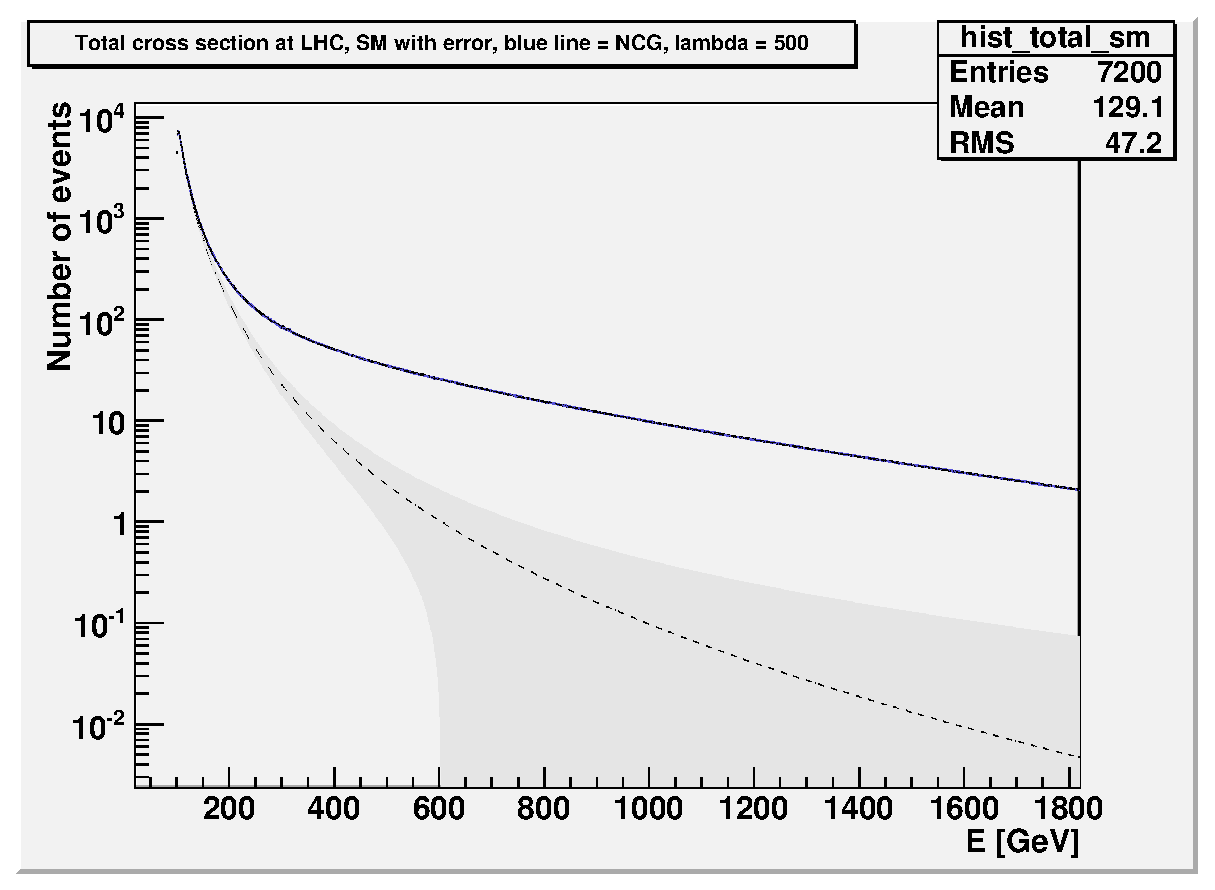
\includegraphics[scale=0.3]{./images/L500r139.eps}
	\end{minipage}
	\hspace{0.3cm}
	\begin{minipage}[b]{0.475\linewidth}
    \centering
	  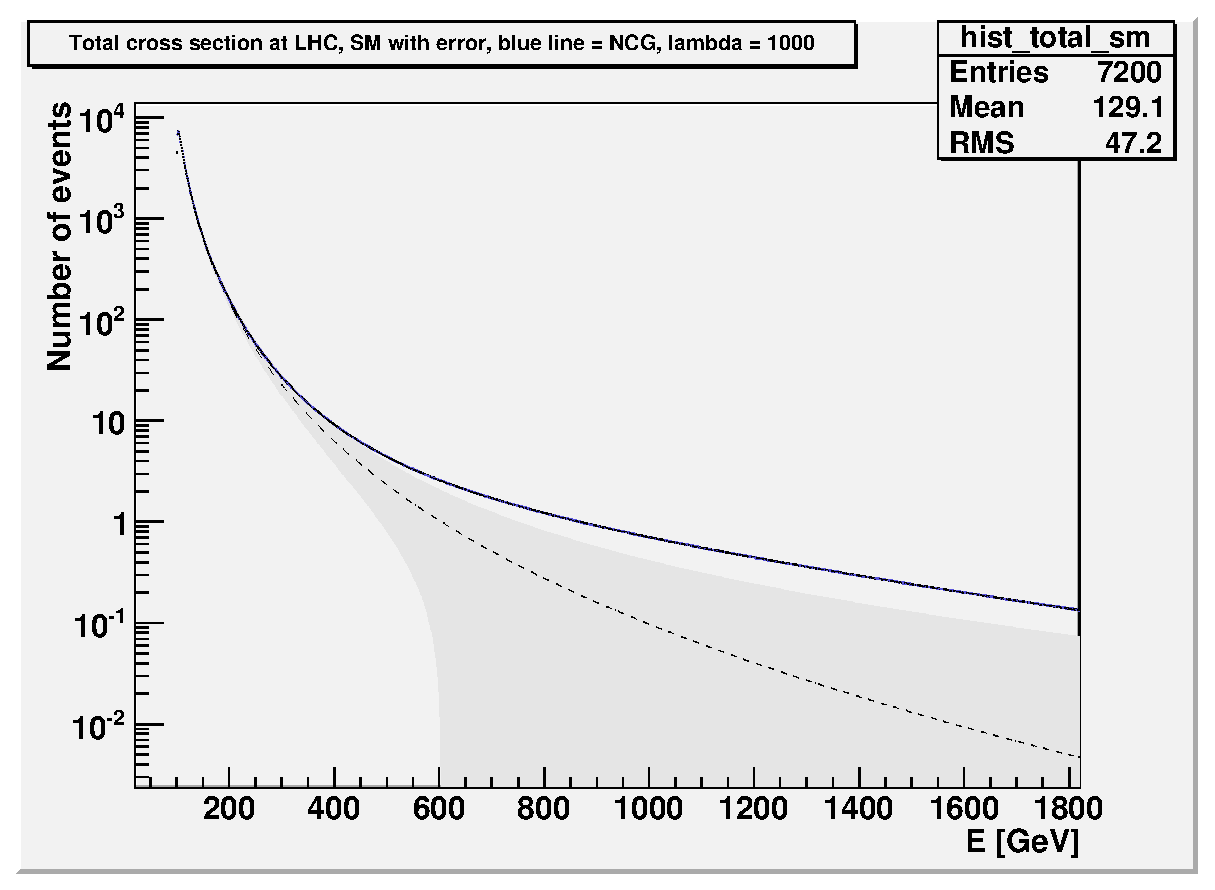
\includegraphics[scale=0.3]{./images/L1000r139.eps}
	\end{minipage}
	\\ \vspace{0.5cm}
	\begin{minipage}[b]{0.475\linewidth}
    \centering
	  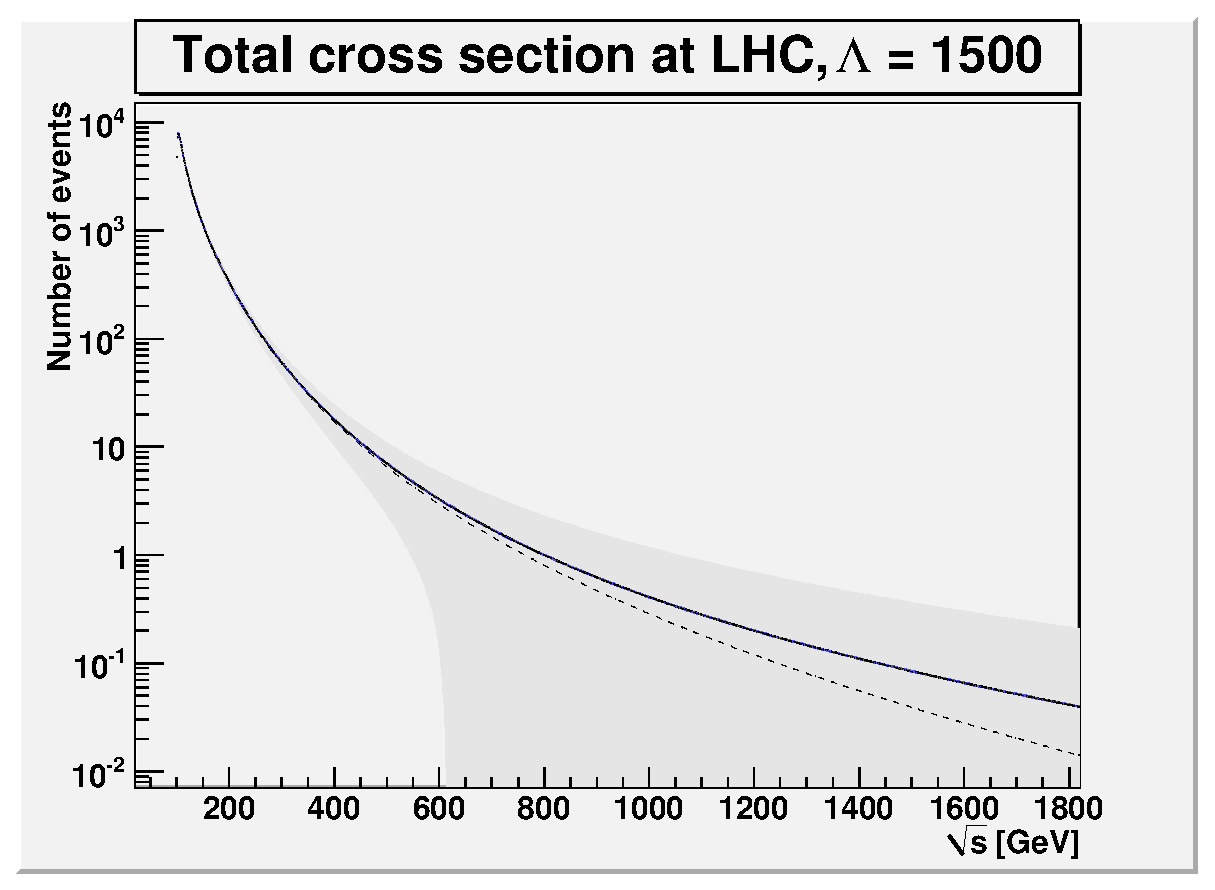
\includegraphics[scale=0.3]{./images/L1500r139.eps}
	\end{minipage}
	\hspace{0.3cm}
	\begin{minipage}[b]{0.475\linewidth}
    \centering
	  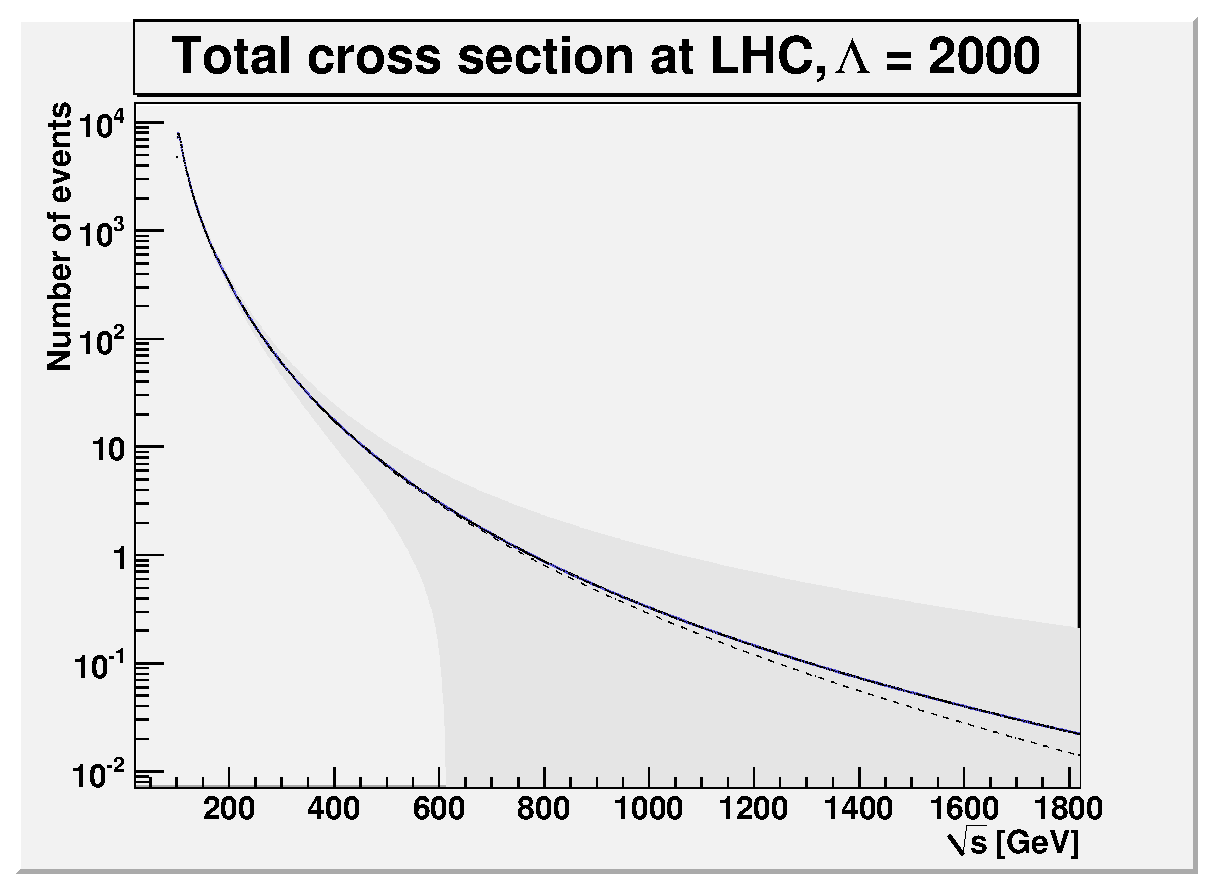
\includegraphics[scale=0.3]{./images/L2000r139.eps}
	\end{minipage}
		\caption{Predicted number of $pp \rightarrow Z/ \gamma \rightarrow \mu \bar \mu$ events at LHC running with a luminosity of $L=10 \textrm{ fb}^{-1}$ for one year. The grey line shows number of events as predicted by the SM with error of $1/\sqrt{N}$, where $N$ is the number of events in the given bin. The blue line represent number of events as predicted by NCG for the given value of $\Lambda$. All interference terms and possible NCG contributions from $\gamma gg$ vertices have been ignored.}\label{fig:lambdaplot}
\end{figure}

% % % % % % % % % % % % % % CONCLUSION % % % % % % % % % % % % % % % % %

\section{Conclusion}
Hopefully LHC will start up this summer and within a few years reach the maximum energy of 14 TeV. The maximum energy currently available is at the Tevatron, and that is only running 2 TeV. The LHC is designed to reach energies of up to 14 TeV, this is a quantum leap in the power available to particle physicists, and may produce results that can one day revolutionize our way of understanding physics on the high energy scales. In either case, LHC may be able to give us a hint as to which direction we should work. In our bachelor project we have worked with Non-commutative geometry, one of the many proposed extensions to the SM. It have mostly been a literarily study of the, not so familiar, subject. We have builded, step by step, a fundament for understanding how QFT, GR, the SM, CompHEP and ROOT work together to produce predictions in HEP. Using these tools we have come to conclusions regarding the visibility of NCG at the LHC.

By using data from LEP we have been able to put a lower limit on the scale at which NCG could become visible. In the case of maximal interaction we have found this limit to be $\Lambda > 117$ GeV, see figure \ref{fig:kplot}.

Furthermore we have studied muon pair-production at the LHC using numerical tools to make several histograms of the total cross section including NCG contributions. Compared to what we expect from ordinary SM calculations the NCG cross section have been shown to become visible above the statistical uncertainty for $\Lambda < 500$, see Figure \ref{fig:lambdaplot}. Given that we do not detect any anomaly in the cross section for pair production when LHC probes the given energies, we can put a lower limit on $\Lambda$ of the order $\Lambda > 1000$ GeV. This is compatible with studies previously made by P. L. Rosendahl \cite{rosendahl2008}, who put a limit $\Lambda_{Rosen} > 2319 GeV$.

If we should actually detect an increase in cross section comparable to what we have seen here, NCG could be one of the explanations that should be look into.

[MAN VIL MAN IKKE KUNNE SE EN SYSTEMATISK FEJL HVIS NCG KURVEN LIGGER LIGE PÅ GRÆNSEN!?]

%What if we actually see a much larger Z cross section at high energy levels? Can we then confirm NCG or could there be other (new) explanations?

%This is not always an easy job. Actually we are in the middle in every sense. In our education, in a course about experimental high energy physics and in the proceeding with LHC at CERN. As we every week gain more knowledge, our level of understanding changes. This makes it difficult to feel like having an overview and sometimes we feel a sudden urge to add all our updated informations.\\

% % % % % % % % % % % % % % % BIBTEX % % % % % % % % % % % % % % % % % %

\clearpage

\bibliographystyle{plain}

% The standard styles distributed with BIBTeX
% alpha	 Sorted alphabetically. Labels are formed from name of author and year of publication with entry labels like "Knu66" formed from the author's name and the year of publication.
% plain	Standard style for producing bibliographies that are sorted alphabetically by author and labeled with numbers.
% unsrt	 Like `plain', but entries are in order of citation. Standard style for producing bibliographies that are labeled with numbers and with entries that appear in the order of their first citation.
% abbrv	 Like `plain', but more compact labels. Standard style for producing bibliographies that are sorted alphabetically by author and labeled with numbers. Author names, month names and journal names are abbreviated.

\bibliography{ncg_citations}		% Navn paa BibTex -filen

\clearpage

%\pagenumbering{Alph}

% % % % % % % % % % % % % % APPENDICES % % % % % % % % % % % % % % % % %

\section{Appendix A}

Lidt om tensor notation og Einstein summation.

\clearpage


\section{Appendix B}
\subsection{Cross Sections}


\clearpage


\section{Appendix C}
Noget om parton distribution functions.

% % % % % % % % % % % % % % SLUT PRUT % % % % % % % % % % % % % % % % % %

\end{document}
